% !TEX root = ../main.tex
%
\chapter{Results}
\label{sec:result}

This section presents the results of the user study conducted to evaluate the usability of the application.
First the results of the quantitative user experience questionnaire are presented, to gauge the overall user experience.
Following this, the results of the qualitative user testing are analyzed, to provide more detailed insights into the usability of the application.
Finally, the results are integrated and discussed.

\section{User Experience Questionnaire}
\label{sec:result:ux}

Even with the relatively small sample size of 10 participants, the results of the User Experience Questionnaire (UEQ) provide a good overview of the overall user experience.
The scores for the different scales of the UEQ are shown in Figure~\ref{fig:ueq-1}. 

\begin{figure}[htb]
	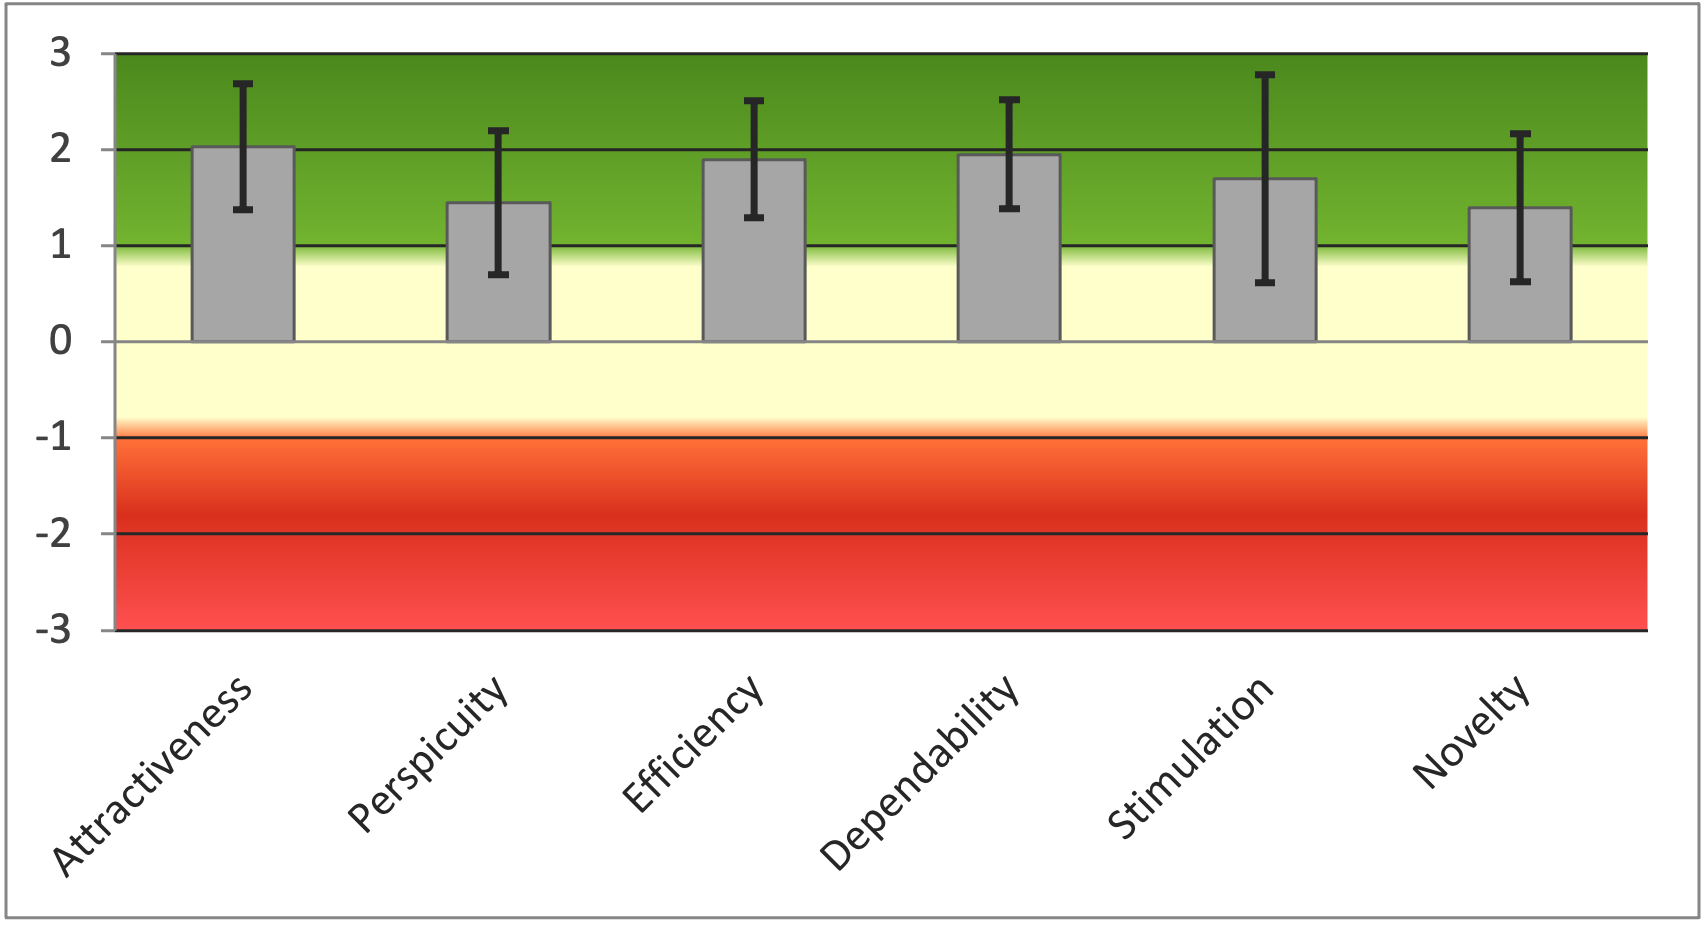
\includegraphics[width=\textwidth]{figures/ueq-1.png}
	\caption{Results of the User Experience Questionnaire}
  \label{fig:ueq-1}
\end{figure}

The \emph{Novelty} scale scores the lowest with a value just below 1 and the \emph{Attractiveness} scale has the highest score with 1.98.
The other scales score between 1.5 and 1.8, indicating a generally positive user experience.

To put the results into perspective, the scores of the UEQ can be benchmarked against the results of other studies.
The UEQ provides a benchmark containing the results of 452 other studies. 
The benchmarking results of the UEQ are shown in Figure~\ref{fig:ueq-2}.
\emph{Attractiveness} and \emph{Dependability} classify as \emph{Excellent}, placing them in the top 10\% of all studies.
\emph{Stimulation} and \emph{Efficiency} both are classified as \emph{Good}, while \emph{Novelty} and \emph{Perspicuity} only classify as \emph{Above Average}.

\begin{figure}[htb]
	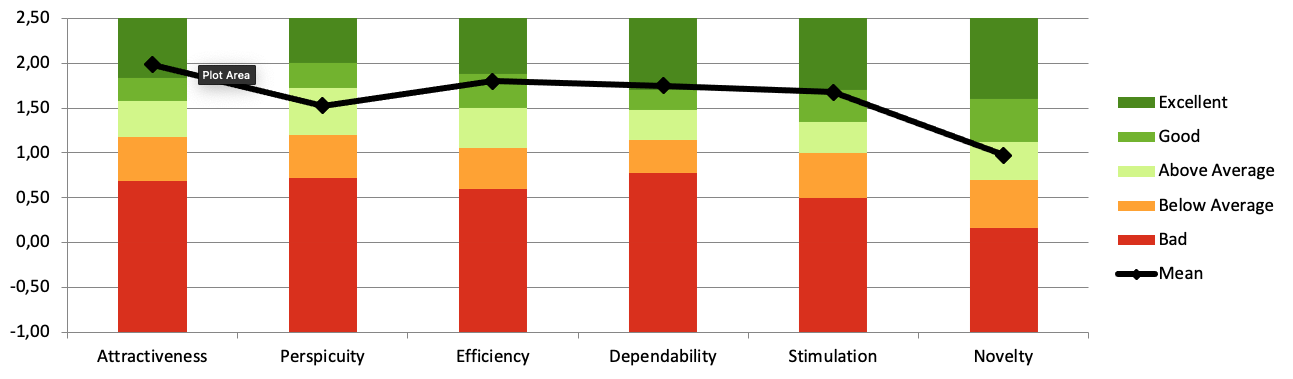
\includegraphics[width=\textwidth]{figures/ueq-2.png}
  \caption{Benchmarking Results of the User Experience Questionnaire}
  \label{fig:ueq-2}
\end{figure}

% TODO: specify relation between variance and confidence interval
The variance of the scores is relatively high, due to the small sample size.
Across the first five scales it is between 0.49 and 0.92, only exceeding 1 for the \emph{Novelty} scale with a value of 1.31.

Table \ref{tab:ueq-summary} provides a summary of the results of the UEQ, besides the mean values and confidence intervals, shown in Figure \ref{fig:ueq-1}, it also includes the standard deviation.
The standard deviation can be interpreted as a measure of agreement between the participants, with lower values indicating higher agreement.
Any value below 0.83 is considered \emph{high agreement}, while values between 0.83 and 1.01 are considered \emph{medium agreement} and values above 1.01 are considered \emph{low agreement}.
Of the six scales, three have a high agreement, two have a medium agreement and one has a low agreement.

\begin{table}[htb]
  \centering
  \begin{tabularx}{\textwidth}{|X|l|l|l|l|l|}
  \hline
      \textbf{Scale} &  \textbf{Mean}  &  \textbf{Conf.} &  \textbf{Conf. Int.} &  \textbf{Std. Dev.} & \textbf{Agreement}\\ \hline
      \textbf{Attractiveness} & 1,983  & 0,445 & 1,538 - 2,428 & 0,718 & high \\ \hline
      \textbf{Perspicuity} & 1,525 & 0,573 & 0,952 - 2,098 & 0,924 & medium\\ \hline
      \textbf{Efficiency} & 1,800 & 0,500 & 1,300 - 2,300 & 0,806 & high \\ \hline
      \textbf{Dependability} & 1,750 & 0,432 & 1,318 - 2,182 & 0,691 & high \\ \hline
      \textbf{Stimulation} & 1,675 & 0,594 & 1,081 - 2,269 & 0,958 & medium \\ \hline
      \textbf{Novelty} & 0,975 & 0,710 & 0,265 - 1,685 & 1,145 & low \\ \hline
  \end{tabularx}
  \vspace{6pt}
  \caption{Summary of the User Experience Questionnaire Results}
  \label{tab:ueq-summary}
\end{table}

\subsection*{Conclusion}

The analysis of the UEQ results gives some insights regarding the application's user experience. 
Higher scores in the \emph{Attractiveness} and \emph{Efficiency} scales, accompanied by high agreement among participants, indicate that these aspects of the application are both effective and appealing. 
The consistency in these scores suggests that such attributes can be quickly gaged by users, even within the limited timeframe of the user study, leading to a uniformly positive perception.

On the other hand, the lower score and agreement on the \emph{Novelty} scale indicate varied perceptions of the application’s innovativeness. 
This could imply that while the application may not introduce new features or functionalities, it effectively repackages existing ones within an intuitive user interface. 
The moderate novelty score might reflect a use of familiar concepts and interactions, which can reduce the learning curve by leveraging well-understood mechanisms.

However, it is important to note that these findings are based on a relatively small sample size of 10 participants. 
While the results provide valuable insights, they should not be overvalued or considered definitive. 
Caution should be exercised in generalizing these findings without further validation from a larger, more diverse sample.

\section{Findings from Qualitative User Testing}
\label{sec:result:testing}
% TODO: Add findings from qualitative user testing


\section{Integration and Findings}
\label{sec:result:findings}
% TODO: Add integration and findings

